\documentclass[../../thesis.tex]{subfiles}

\begin{document}

\section{Implementation details}
We follow \cite{TimeVQVAE} closely in the encoder/decoder/codebook implementation, and 

\subsubsection{Time Frequency Modelling}
The short time fourier transform (STFT) and its inverse ISTFT are implemented with \texttt{torch.stft} and \texttt{torch.istft} respectively. We follow \cite{TimeVQVAE} and set the main parameter \texttt{nfft} to $8$, and use default parameters for the rest. This results in a fequency axis with range $[1,2,3,4,5]$ and half as long time axis. \newline


\subsubsection{Encoder and decoder}

The same encoder and decoder architecture as in \cite{VQVAE} is used and further use the implementation from \cite{nadavbh12} with adaptations from \cite{TimeVQVAE}.\newline

The encoder presented in figure \ref{fig:VQVAE Encoder} consists of $n$ downsampling convolutional blocks (\texttt{Conv2d - BatchNorm2d - LeakyReLU}), followed by $m$ residual blocks (\texttt{LeakyReLU - Conv2d - BatchNorm2d - LeakyReLU - Conv2d}). The downsampling convolutional layers are implemented with parameters: \texttt{kernel size=(3,4),
stride=(1,2), padding=(1,1)}. This results in downsampling of only the temporal axis, which is downsampled by a factor of $2$ for each downsampling block. The residual convolutional layers have parameters: \texttt{kernel size=(3,3),stride=(1,1), padding=(1,1)}.\newline

The decoder is implemented similarity with $m$ residual followed $n$ upsampling layers using transposed convolutional blocks with same parameters as in the encoder.\newline

The downsampling rate is determined by $2^n$ where $n$ is set such that $z$ has width of $32$. For more in depth consideration of the detail regarding TimeVQVAE implementation we refer to Appendix C.3 of \cite{TimeVQVAE}.

\begin{figure}[h]
    \label{fig:VQVAE Encoder}
    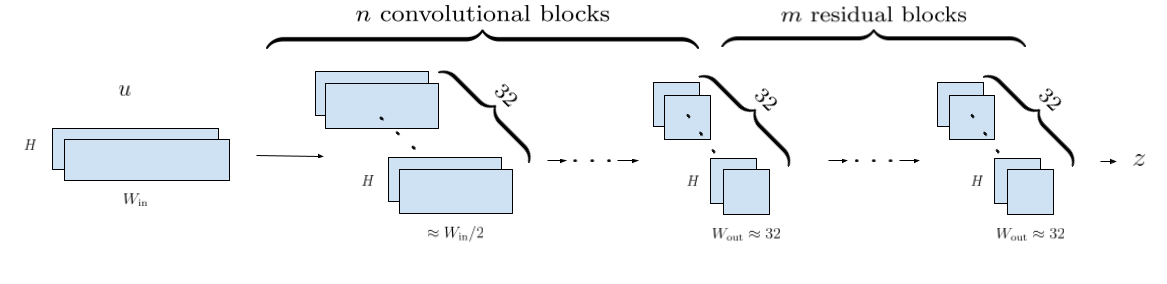
\includegraphics[scale = 0.3]{VQVAE Encoder.png}
    \centering
    \caption{Overview of the encoder architecture. The decoder architecture is simply obtained by reversing the arrows and switching out the convolutional block for transposed convolutional blocks.}
\end{figure}

\subsubsection{VQ}
Implementation from lucidrains/vector-quantize-pytorch. https://github.com/lucidrains/vector-quantize-pytorch \newline
Codebook size = 32 and dimension = 64. \newline
Use exponential moving average with decay $0.9$, and commitment loss with weight $\beta = 1$.

\subsubsection{Augmentations}
window warp:    window ratio: 0.4,min window warp: 0.9, max windowwarp: 2.0\newline
amplitude resize: Amp Rrate: 0.2\newline
gaussian noise: gaus mean: 0, gaus std: 0.05\newline
slice and shuffle:\newline

\subsubsection{Projector}
We follow the implementation from \cite{lee2024computer} for both Barlow Twins and VIbCReg.\newline
Barlow Twins: Projector's dimension size is set to $4096$. $\lambda$ is set to $5\cdot10^3$. \newline
VIbCReg: The dimension of the the projector is set to $4096$. $\lambda$ and $\mu$ are both set to $25$, while $\nu$ is set to $100$.

\subsubsection{Prior learning}
The number of iterations in the iterative decoding algorithm $T$, is set to $10$, following \cite{chang2022maskgit}. We too use the cosine as mask scheduling function $\gamma$. The implementation is adopted from \cite{TimeVQVAE}. 


\subsubsection{Optimizer}
The AdamW optimizer with batch sizes for stage1: 128 and stage2: 256, initial learning rate $10^{-3}$, cosine learning rate scheduler and weight decay of $10^{-5}$. We run 1000 epochs for both stage 1 and 2. 

\subsubsection{Evaluation}
KNN and SVM are implemented using scikit-learn. $K=5$ in KNN and linear kernel in SVM.\newline
FCN for IS, FID and CAS

\section{Initial Experimentation and Model Development}

The overarching objective in creating our model is to learn more expressive latent representations for better time series generation. We want to improve the reconstruction capabilities of the tokenization model. The rationality is that if the tokenization model reconstructs well the latent representations contains all relevant information of the input. We simultaneously want enforce better class separability in the latent representations, as we hypothesize that such additional structure eases/improved learning of the generative model.\newline

During development we encountered several problems:\newline
When we attempted a siamese architecture, with quantization in the augmented branch, and to derive the SSL loss from the discrete representations there were a correlation problem. The codewords were very highly correlated, which resulted from the passing both views through the VQ.  $SSL(z_q,z_q')$ \newline
In an attempt to solve this we attempted to derive the SSL loss from the continuous latent representations, but the resulting discrete latent representations performed poorly on the downstream classification task. Separability problem: $SSL(z,z')$ \newline
The solution was to remove the VQ in the augmented branch and rather derive the SSL loss from $z_q$ and $z'$. Solution: $SSL(z_q,z')$ \newline

Overfitting problem: Using $SG()$ on augmented branch / Not using augRecons \newline

\section{Main Experiments}

We are primarily interested in two things. For stage 1, if NC-VQVAE learns more expressive representations, i.e are we able to reconstruct on par with VQVAE while simultaneously improve on downstream classification. For stage 2 we are interested in the effect NC-VQVAE has on prior learning and time series generation. \newline

We evaluate our model NC-VQVAE with both Barlow Twins and VIbCReg as SSL method against the naive VQVAE as described in \cite{TimeVQVAE}. For each SSL method, we train three separate models which uses different sets of augmentations. Firstly we look at the tokenization models, evaluating the reconstruction capability and performance on downstream classification. Then we train a prior model on top of the different tokenization models and evaluate the performance of the generative models by IS, FID, CAS and visual inspection.\newline


\section{Stage 1}

\subsection{Augmentations}
In our experiments we consider three sets of augmentations with different characteristics. They are
\begin{itemize}
    \item Amplitude Resizing + Window Warp
    \item Slice and Shuffle
    \item Gaussian noise
\end{itemize}

\textbf{Amplitude Resizing + Window Warp} scales in both x and y direction. The window warp has similar qualities to phase shift, but not uniformly and keeps endpoints fixed. They were considered as the observed conditional distribution in some datasets, such as ShapesALL \ref{fig:datasets}, had similar overall shape, but peaked with different amplitude and at different locations. Thus the augmented view had similar characteristics as the conditional distribution of the original view \ref{fig:ShapesAll_winwarp}. \newline

\begin{figure}[h]
    \label{fig:ShapesAll_winwarp}
    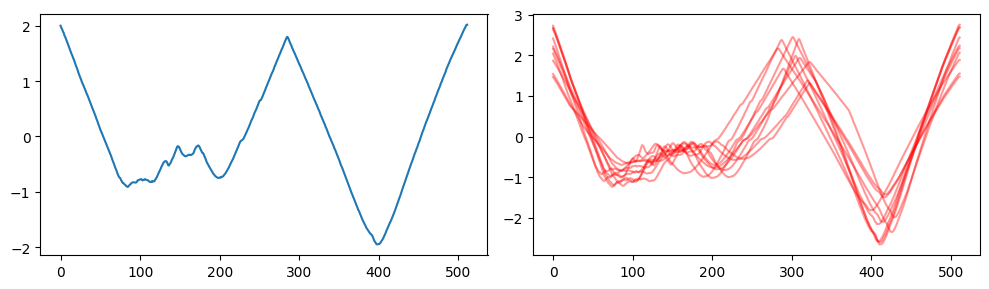
\includegraphics[scale = 0.3]{ShapesAll_winwarp.png}
    \centering
    \caption{ShapesAll: Original (left), augmented (right). 15 instances of Amplitude Resizing + Window Warp applied to the original sample.}
\end{figure}

\textbf{Slice and Shuffle} crops the time series into four sections and permutes them. For datasets with sharp modularity and few peaks, such as ElectricDevices \ref{fig:datasets}, the augmentation provides a view with peaks occurring at timestamps not seen in the training data, which is illustrated in figure \ref{fig:ElectricDevices_SliceAndShuffel}. This could improve the reconstruction on unseen data, as well as encouraging the model to focus more on the existence of a peak rather than its specific location. For some datasets such as FordA \ref{fig:datasets}, the semantics of the dataset is preserved under this augmentation, despite their continuous nature.\newline
\begin{figure}[h]
    \label{fig:ElectricDevices_SliceAndShuffel}
    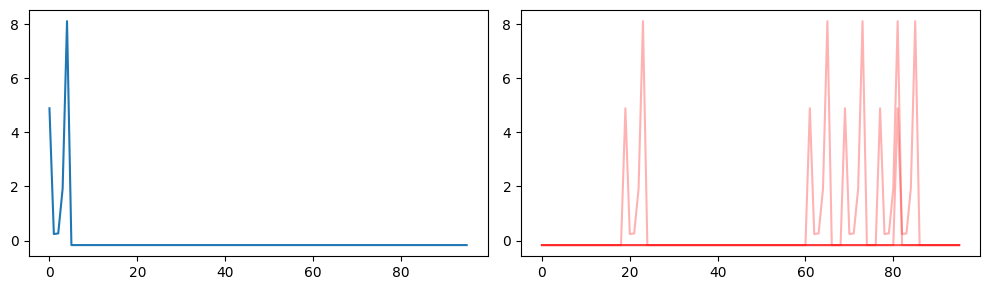
\includegraphics[scale = 0.3]{ElectricDevices_SliceAndShuffel.png}
    \centering
    \caption{ElectricDevices: Original (left), augmented (right). 5 instances of Slice and Shuffle applied to the original sample.}
\end{figure}


\textbf{Gaussian noise} adds a nose $\epsilon \sim N(0,0.05)$ to each datapoint in the time series. This introduces, in many cases, a substantial high frequency component as seen in figure \ref{fig:StarLight_Gaussian}. As the naive VQVAE described in \cite{TimeVQVAE} had trouble with reconstruction of HF components, this augmentation could provide more emphasis on these. The reconstruction of the augmented views can too provide more information regarding HF components for the decoder. Of the three augmentations, gaussian noise provides the most predictable augmented views from a numerical standpoint, which might result in a SSL loss which is easier to minimize.

\begin{figure}[h]
    \label{fig:StarLight_Gaussian}
    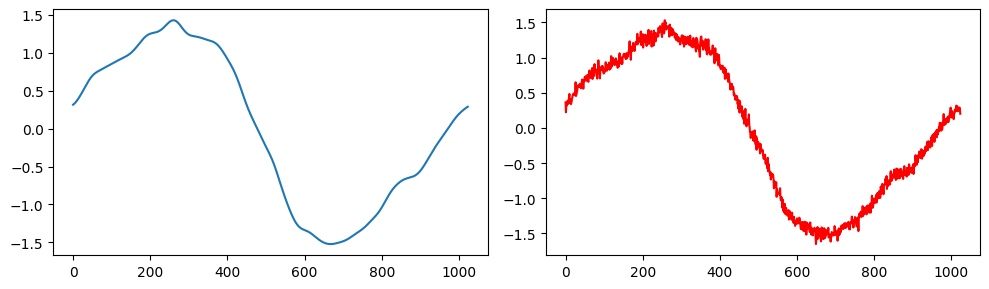
\includegraphics[scale = 0.3]{StarLight_Gaussian.png}
    \centering
    \caption{StarLightCurves: Original (left), augmented (right). One instance of Gaussian noise applied to the original sample.}
\end{figure}

\subsection{Evaluation}
Reconstruction, Classification and Visual inspection



\section{Stage 2}

\subsection{Evaluation}

\begin{itemize}
    \item \textbf{IS}:
    \item \textbf{FID}:
    \item \textbf{CAS}:We evaluate the CAS for TSTR by using the Supervised FCN on all our models considered and compare against the baseline model to investigate the relative performance. 
    \item \textbf{Visual inspection}:
    \item \textbf{Token usage}:
\end{itemize}


\section{UCR Time Series Classification Archive}
The evaluation of our model NC-VQVAE is done on a subset of the UCR Time Series Archive \cite{UCRArchive2018}. The UCR archive is a collection of 128 datasets of univariate time series for time series classification. The different datasets in the archive span a wide range characteristics and include among others sensor, device, image-derived and simulated data. Each dataset has a predefined training and test split.\newline

Our subset of the UCR archive is

\begin{table}[h]
    \centering
    \begin{tabular}{llllll}
    \toprule
    Type      & Name                    & Train & Test & Class & Length \\
    \midrule
    Device    & ElectricDevices         & 8926  & 7711 & 7     & 96     \\
    Sensor    & FordB                   & 3636  & 810  & 2     & 500    \\
    Sensor    & FordA                   & 3601  & 1320 & 2     & 500    \\
    Sensor    & Wafer                   & 1000  & 6164 & 2     & 152    \\
    Simulated & TwoPatterns             & 1000  & 4000 & 4     & 128    \\
    Sensor    & StarLightCurves         & 1000  & 8236 & 3     & 1024   \\
    Motion    & UWaveGestureLibraryAll  & 896   & 3582 & 8     & 945    \\
    ECG       & ECG5000                 & 500   & 4500 & 5     & 140    \\
    Image     & ShapesAll               & 600   & 600  & 60    & 512    \\
    Simulated & Mallat	                & 55	& 2345 & 8	   & 1024   \\
    Image     & Symbols                 & 25    & 995  & 6     & 398    \\
    Sensor    & SonyAIBORobotSurface2   & 27    & 953  & 2     & 65     \\
    Sensor    & SonyAIBORobotSurface1   & 20    & 601  & 2     & 70     \\
    \bottomrule
    \end{tabular}
    \caption{The subset of the UCR Archive considered for our experiments.}
    \label{tab:UCRsubset}
    \end{table}

We choose to test on a subset, rather than on the entire UCR Archive, due to computational limitations as well as to more thoroughly investigate the effect of our models and the role of augmentations. The subset is chosen such that they span a wide range of train set sizes, lengths, classes and type, while the class distributions have visually different characteristics which can be seen from table \ref{tab:UCRsubset} and figure \ref{fig:datasets}. 

    \begin{figure}[h]
        \label{fig:datasets}
        \centering
        \begin{minipage}[b]{0.32\textwidth}
            \centering
            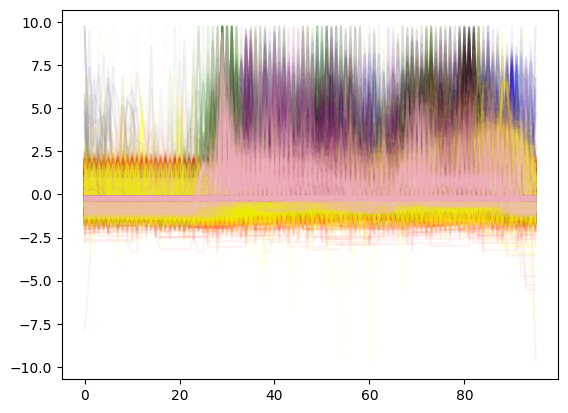
\includegraphics[width=\textwidth]{ElectricDevices}
            \caption*{ElectricDevices}
        \end{minipage}
        \hfill
        \begin{minipage}[b]{0.32\textwidth}
            \centering
            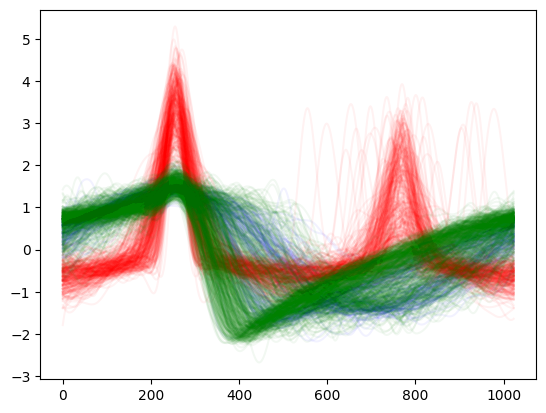
\includegraphics[width=\textwidth]{StarLightCurves}
            \caption*{StarLightCurves}
        \end{minipage}
        \hfill
        \begin{minipage}[b]{0.32\textwidth}
            \centering
            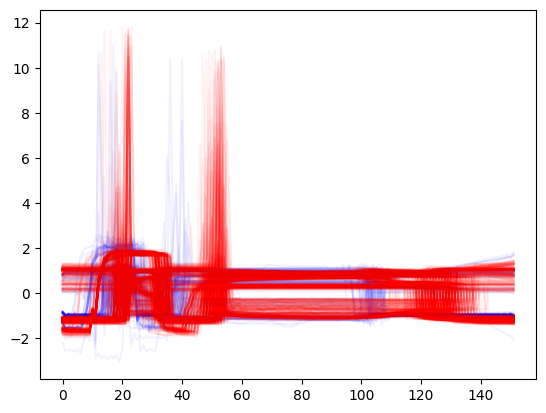
\includegraphics[width=\textwidth]{Wafer}
            \caption*{Wafer}
        \end{minipage}
        
        \vspace{0.4cm}
        
        \begin{minipage}[b]{0.32\textwidth}
            \centering
            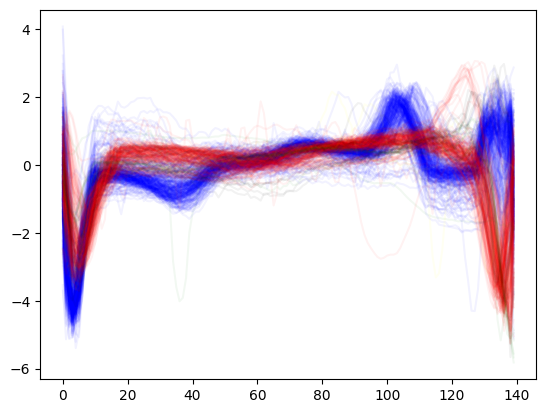
\includegraphics[width=\textwidth]{ECG5000}
            \caption*{ECG5000}
        \end{minipage}
        \hfill
        \begin{minipage}[b]{0.32\textwidth}
            \centering
            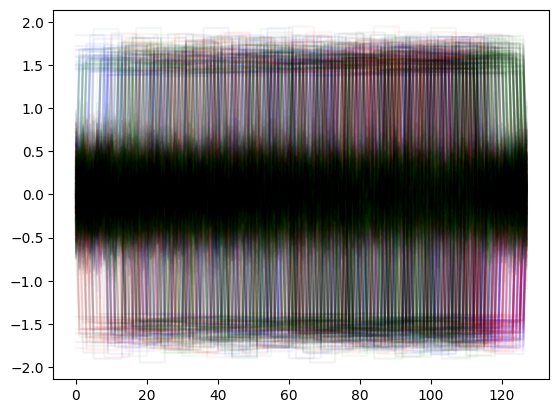
\includegraphics[width=\textwidth]{TwoPatterns}
            \caption*{TwoPatterns}
        \end{minipage}
        \hfill
        \begin{minipage}[b]{0.32\textwidth}
            \centering
            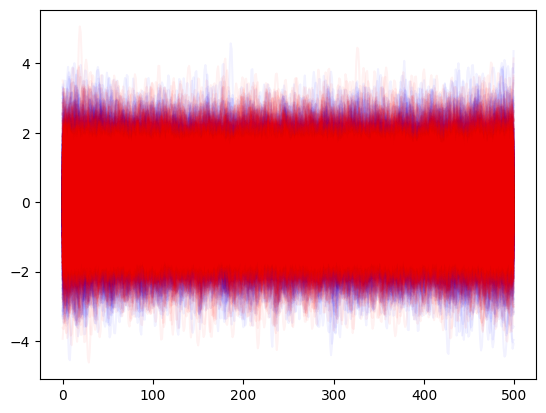
\includegraphics[width=\textwidth]{FordA}
            \caption*{FordA}
        \end{minipage}
        
        \vspace{0.4cm}
        
        \begin{minipage}[b]{0.32\textwidth}
            \centering
            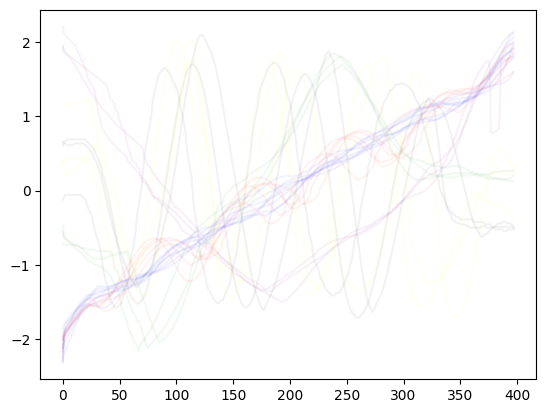
\includegraphics[width=\textwidth]{Symbols}
            \caption*{Symbols}
        \end{minipage}
        \hfill
        \begin{minipage}[b]{0.32\textwidth}
            \centering
            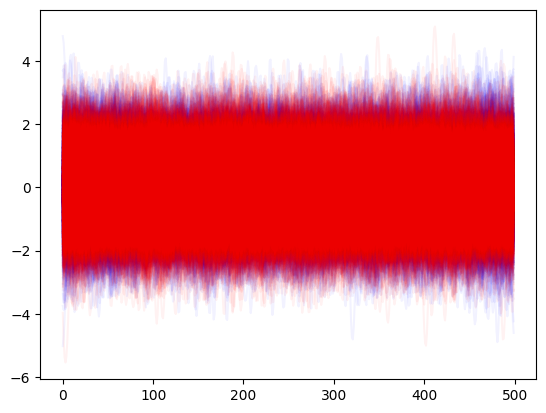
\includegraphics[width=\textwidth]{FordB}
            \caption*{FordB}
        \end{minipage}
        \hfill
        \begin{minipage}[b]{0.32\textwidth}
            \centering
            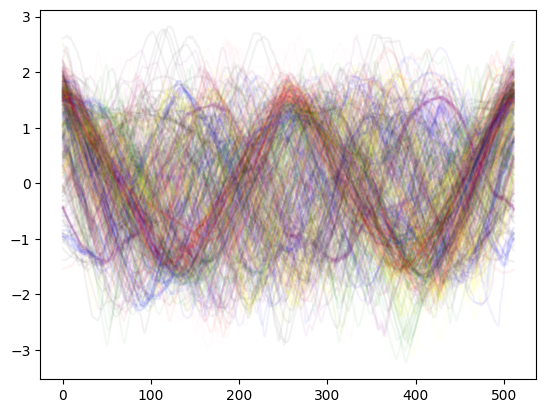
\includegraphics[width=\textwidth]{ShapesAll}
            \caption*{ShapesAll}
        \end{minipage}
        
        \vspace{0.4cm}
        
        \begin{minipage}[b]{0.32\textwidth}
            \centering
            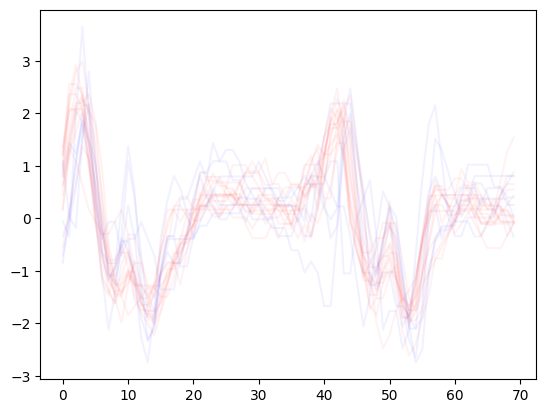
\includegraphics[width=\textwidth]{Sony1}
            \caption*{SonyAIBORobotSurface1}
        \end{minipage}
        \hfill
        \begin{minipage}[b]{0.32\textwidth}
            \centering
            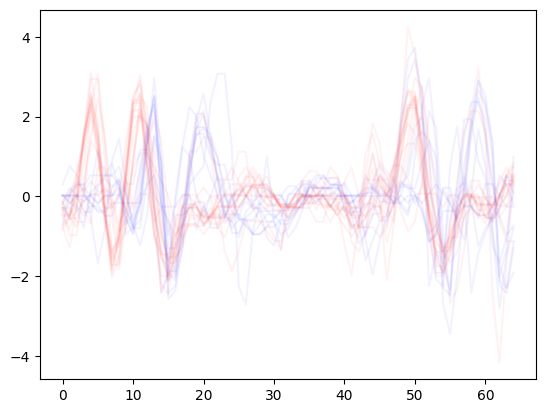
\includegraphics[width=\textwidth]{Sony2}
            \caption*{SonyAIBORobotSurface2}
        \end{minipage}
        \hfill
        \begin{minipage}[b]{0.32\textwidth}
            \centering
            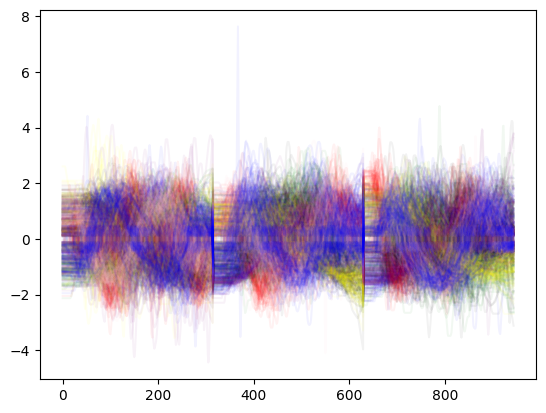
\includegraphics[width=\textwidth]{UWave}
            \caption*{UWaveGestureLibraryAll}
        \end{minipage}
        
        \vspace{0.4cm}
        
        \begin{minipage}[b]{0.32\textwidth}
            \centering
            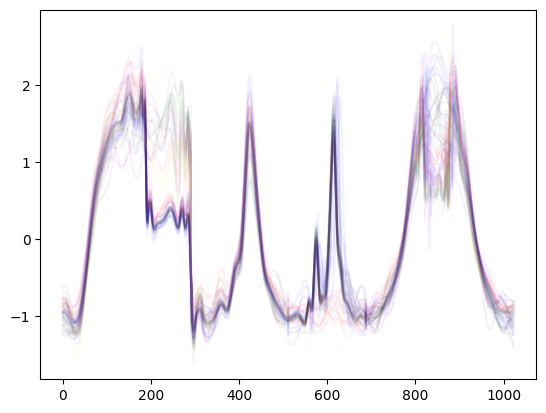
\includegraphics[width=\textwidth]{Mallat}
            \caption*{Mallat}
        \end{minipage}
        
    \end{figure}






\end{document}